\documentclass[]{article}
\usepackage{graphicx}

%opening
\title{Evaluación práctica}
\author{David Alonso Garduño Granados}

\begin{document}

\maketitle

\begin{abstract}
Para lograr que el documento de LaTeX compilara observé que no tenía algunas bibliotecas instaladas en mi computadora personal, observé algunos "Usepackage"y ví que "stackengine" no la había instalado en ninguna de las ocasiones en las que había usado LaTeX con anterioridad, así que fui a la terminal y ejecuté "sudo dnf install texlive-stackengine":
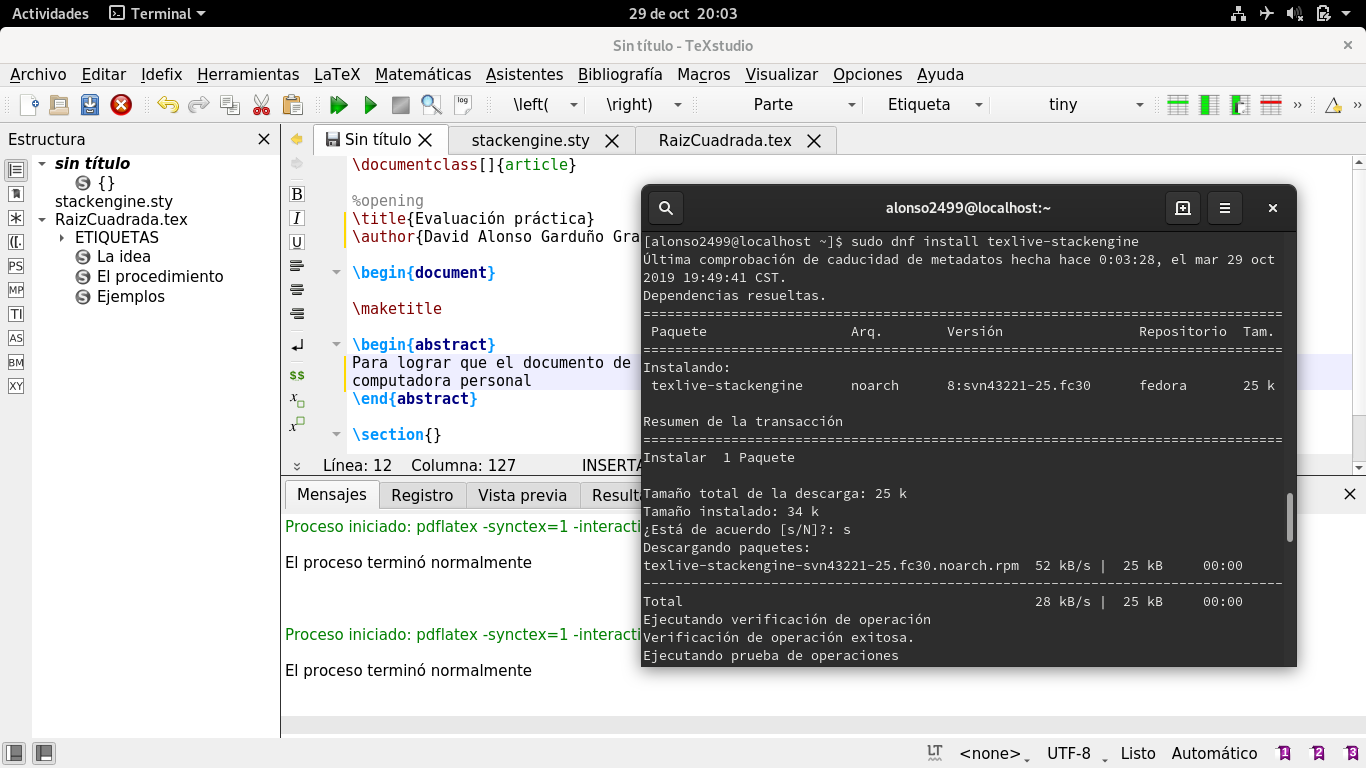
\includegraphics[scale=0.20]{Imagenes/Stackengine.png}

Además otra biblioteca faltante era "listofitems", también la instalé usando la terminal:

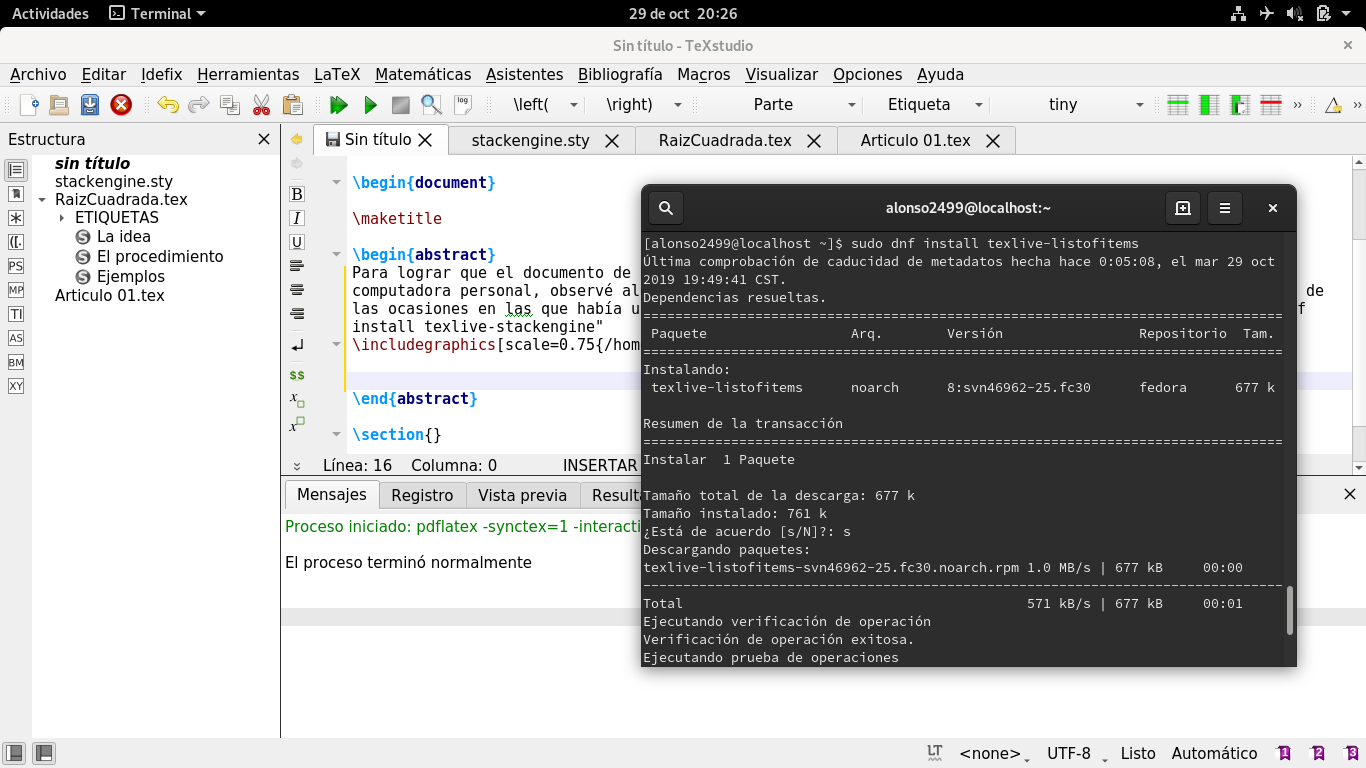
\includegraphics[scale=0.20]{Imagenes/2da.png}
\end{abstract}
\end{document}
